\subsection{Tinyworld}\label{secc:tinyworld}
The Tinyworld is constructed so that for three or more agents, the entire feasible space is covered regardless of the position of the agents.

\Cref{fig:3_agnt_tw_k_1_0_distr} shows the initial and final configuration of 3 agents when spawned in the Tinyworld environment, 
and no active dispersion is used ($k_{1} = 0$).
\Cref{fig:3_agnt_tw_evolution} shows the covered area and step length per agent versus iteration count.

Results of optimizing agent positions with active dispersion ($k_{1} = 1$, $k_{2} = 1$) are shown in \Cref{fig:3_agnt_tw_k_1_1_k_2_1_distr} and \Cref{fig:3_agnt_tw_evolution_active}.

\begin{figure}[H]
  \centering
  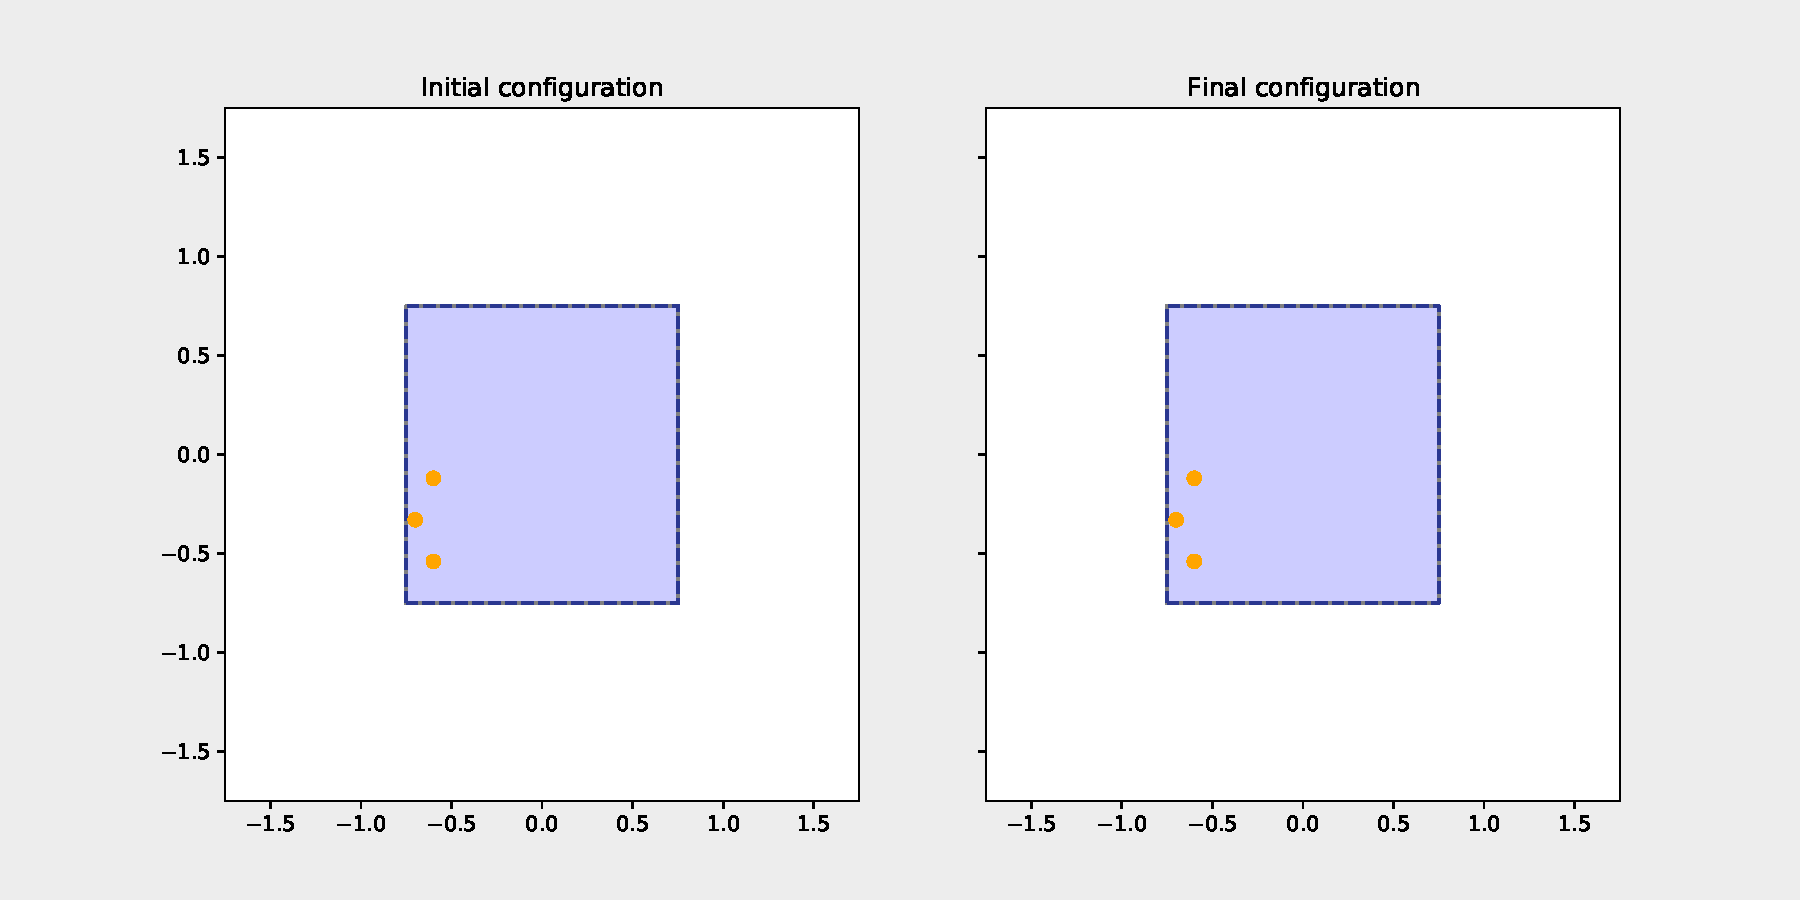
\includegraphics[width=\textwidth]{figs/tinyworld_3_agnt_k_1_0_k_2_1_distr.pdf}
  \caption{Initial and final configuration of 3 agents in the Tinyworld environment with $k_{1} = 0$ (no active dispersion).}
  \label{fig:3_agnt_tw_k_1_0_distr}
\end{figure}

\begin{figure}[H]
  \centering
  \begin{subfigure}[t]{0.5\textwidth}
    \centering
    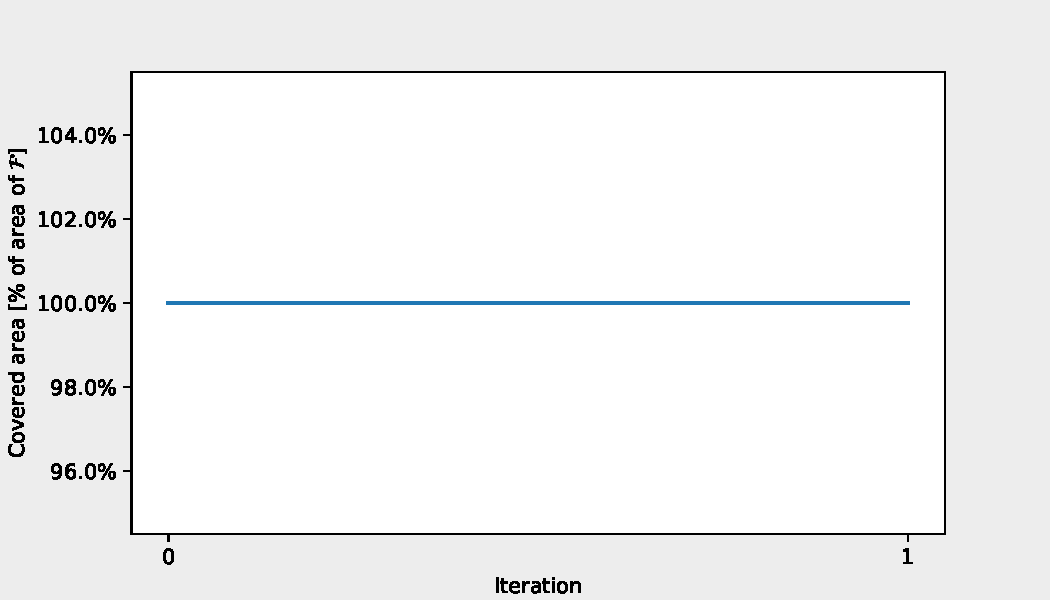
\includegraphics[width=\textwidth]{figs/tinyworld_3_agnt_k_1_0_k_2_1_area_traj.pdf}
    \caption{Coverage evolution for 3 agents in the Tinyworld environment with $k_{1} = 0$ (no active dispersion).}
    \label{fig:3_agnt_tw_k_1_0_a_traj}
  \end{subfigure}%
  ~ 
  \begin{subfigure}[t]{0.5\textwidth}
    \centering
    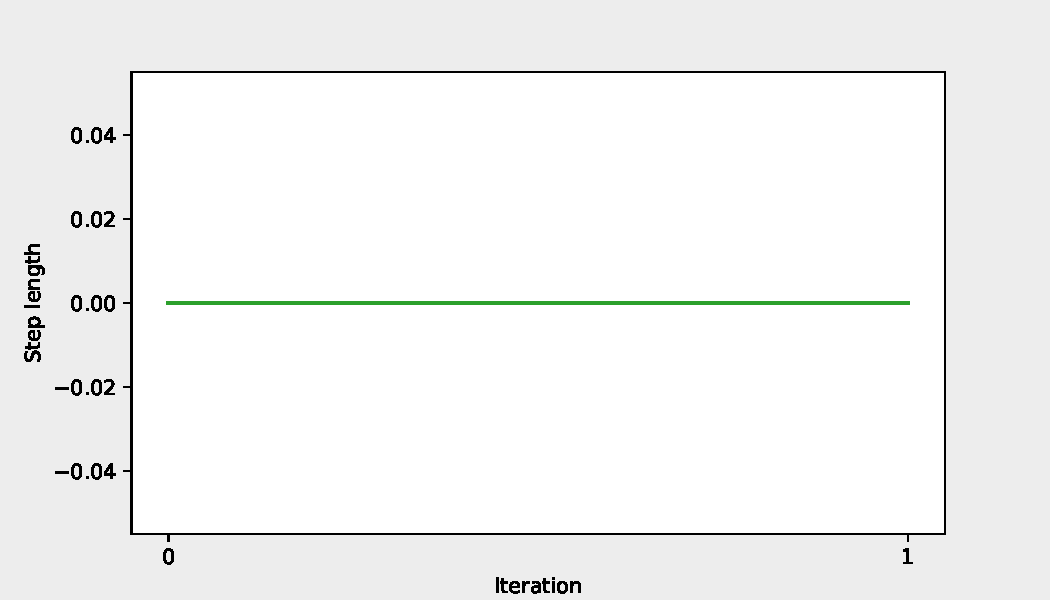
\includegraphics[width=\textwidth]{figs/tinyworld_3_agnt_k_1_0_k_2_1_step_traj.pdf}
    \caption{Step length evolution for 3 agents in the Tinyworld environment with $k_{1} = 0$ (no active dispersion).}
    \label{fig:3_agnt_tw_k_1_0_s_traj}
  \end{subfigure}
  \caption{Coverage percentage and step length evolution for 3 agents in the Tinyworld environment when no active dispersion is used.}
  \label{fig:3_agnt_tw_evolution}
\end{figure}

\begin{figure}[H]
  \centering
  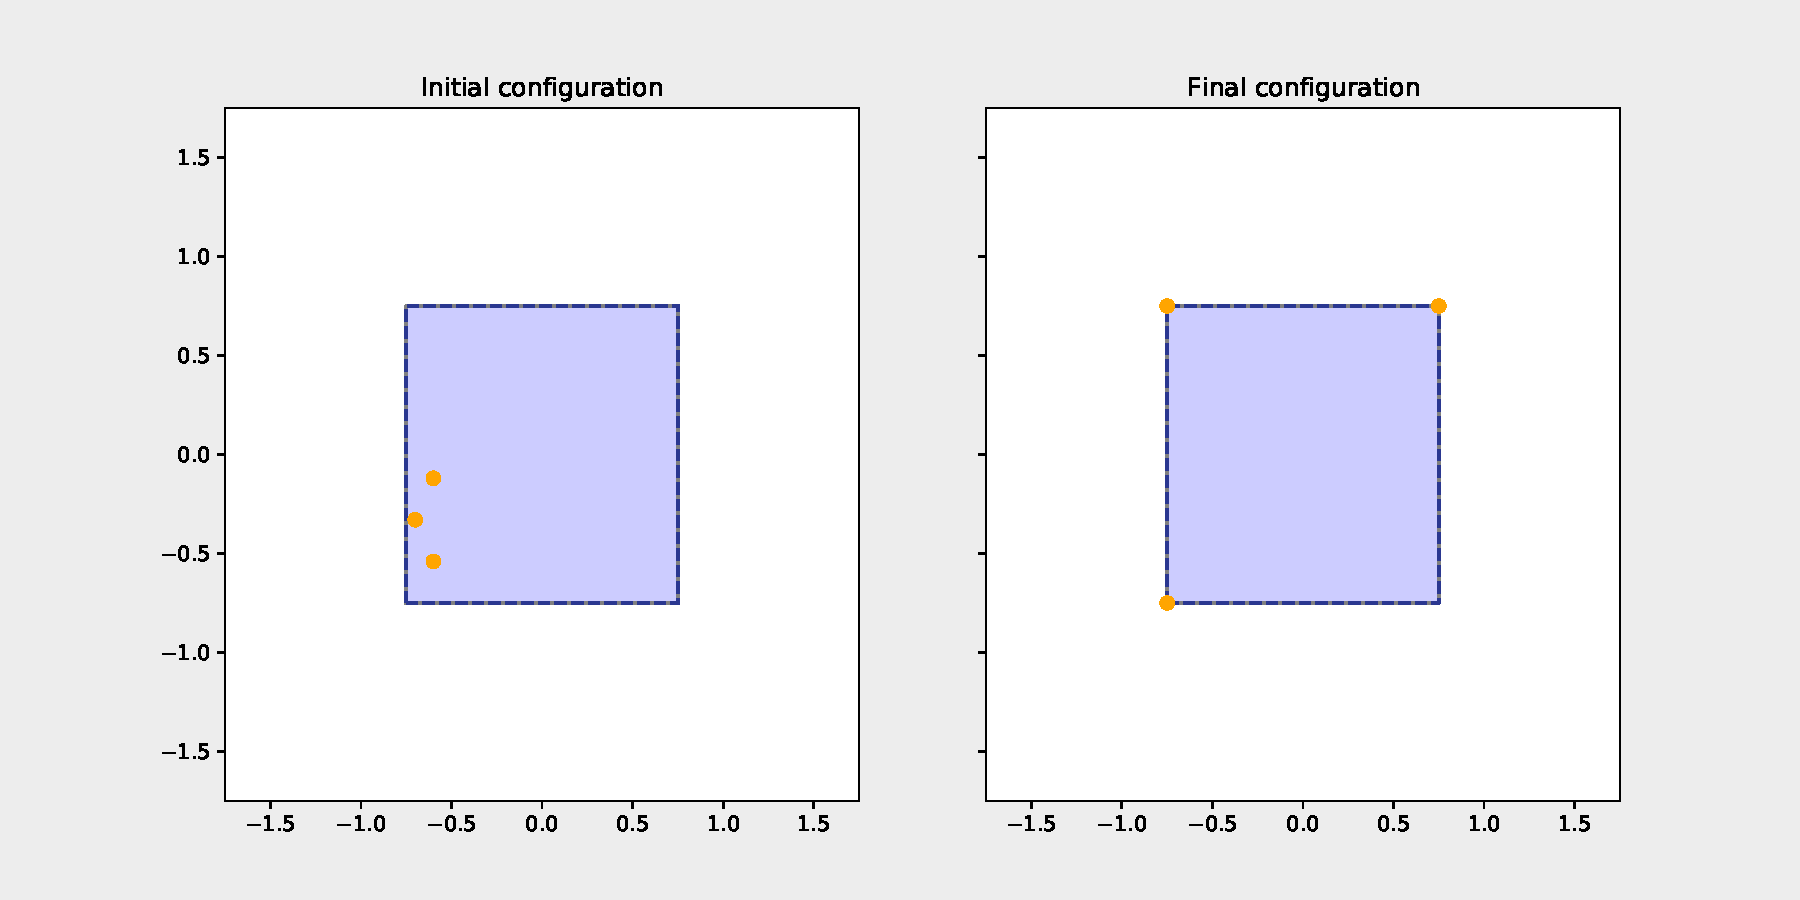
\includegraphics[width=\textwidth]{figs/tinyworld_3_agnt_k_1_1_k_2_1_distr.pdf}
  \caption{Initial and final configuration of 3 agents in the Tinyworld environment with $k_{1} = k_{2} = 1$ (active dispersion).}
  \label{fig:3_agnt_tw_k_1_1_k_2_1_distr}
\end{figure}

\begin{figure}[H]
  \centering
  \begin{subfigure}[t]{0.5\textwidth}
    \centering
    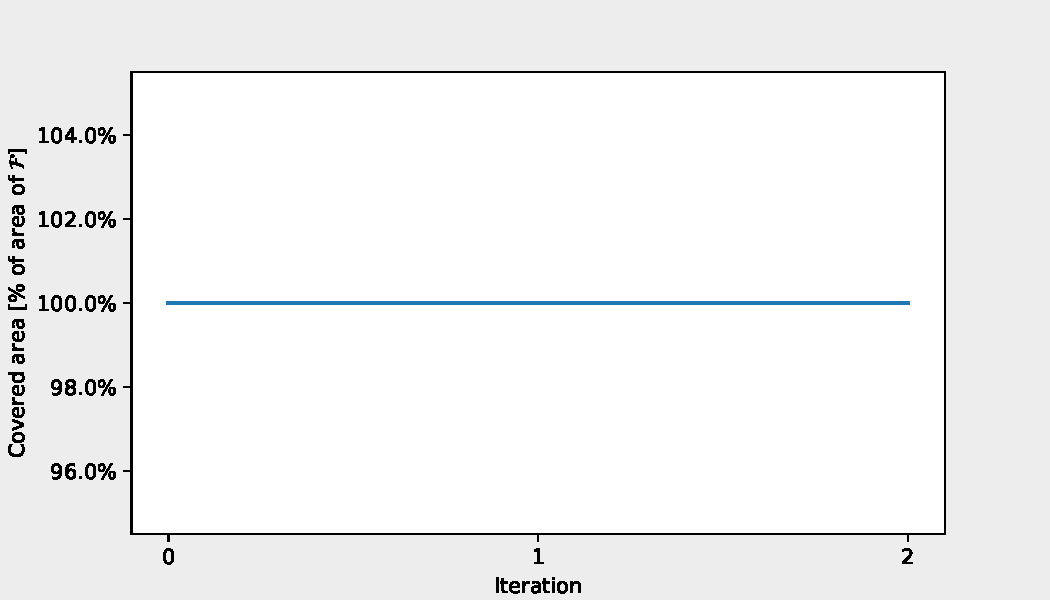
\includegraphics[width=\textwidth]{figs/tinyworld_3_agnt_k_1_1_k_2_1_area_traj.pdf}
    \caption{Coverage evolution for 3 agents in the Tinyworld environment with $k_{1} = k_{2} = 1$ (active dispersion).}
    \label{fig:3_agnt_tw_k_1_k_2_1_a_traj}
  \end{subfigure}%
  ~ 
  \begin{subfigure}[t]{0.5\textwidth}
    \centering
    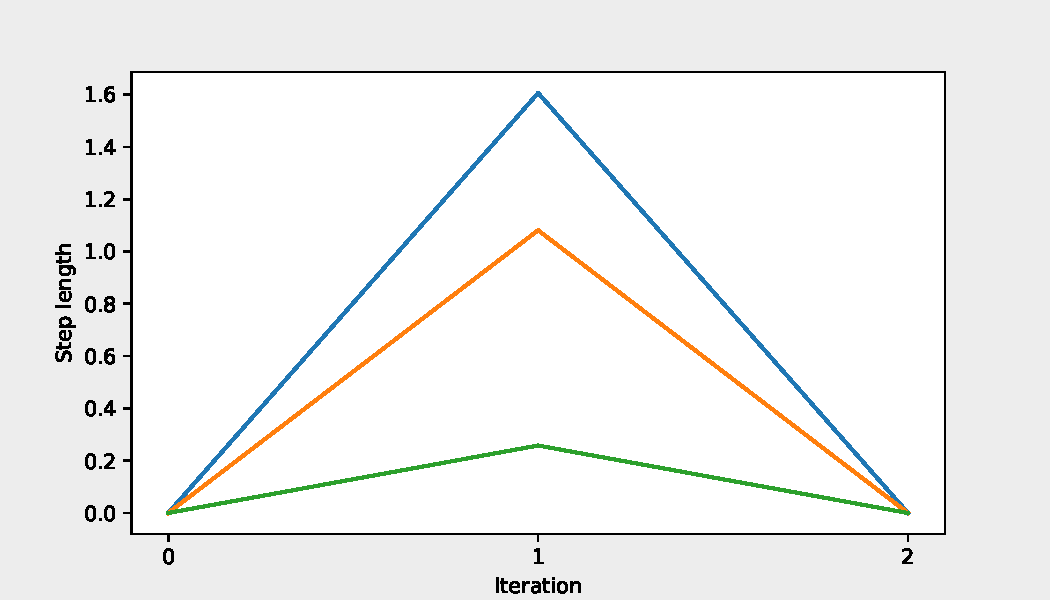
\includegraphics[width=\textwidth]{figs/tinyworld_3_agnt_k_1_1_k_2_1_step_traj.pdf}
    \caption{Step length evolution for 3 agents in the Tinyworld environment with $k_{1} = k_{2} = 1$ (active dispersion).}
    \label{fig:3_agnt_tw_k_1_k_2_1_s_traj}
  \end{subfigure}
  \caption{Coverage percentage and step length evolution for 3 agents in the Tinyworld environment when active dispersion is used.}
  \label{fig:3_agnt_tw_evolution_active}
\end{figure}